\documentclass[1p]{elsarticle_modified}
%\bibliographystyle{elsarticle-num}

%\usepackage[colorlinks]{hyperref}
%\usepackage{abbrmath_seonhwa} %\Abb, \Ascr, \Acal ,\Abf, \Afrak
\usepackage{amsfonts}
\usepackage{amssymb}
\usepackage{amsmath}
\usepackage{amsthm}
\usepackage{scalefnt}
\usepackage{amsbsy}
\usepackage{kotex}
\usepackage{caption}
\usepackage{subfig}
\usepackage{color}
\usepackage{graphicx}
\usepackage{xcolor} %% white, black, red, green, blue, cyan, magenta, yellow
\usepackage{float}
\usepackage{setspace}
\usepackage{hyperref}

\usepackage{tikz}
\usetikzlibrary{arrows}

\usepackage{multirow}
\usepackage{array} % fixed length table
\usepackage{hhline}

%%%%%%%%%%%%%%%%%%%%%
\makeatletter
\renewcommand*\env@matrix[1][\arraystretch]{%
	\edef\arraystretch{#1}%
	\hskip -\arraycolsep
	\let\@ifnextchar\new@ifnextchar
	\array{*\c@MaxMatrixCols c}}
\makeatother %https://tex.stackexchange.com/questions/14071/how-can-i-increase-the-line-spacing-in-a-matrix
%%%%%%%%%%%%%%%

\usepackage[normalem]{ulem}

\newcommand{\msout}[1]{\ifmmode\text{\sout{\ensuremath{#1}}}\else\sout{#1}\fi}
%SOURCE: \msout is \stkout macro in https://tex.stackexchange.com/questions/20609/strikeout-in-math-mode

\newcommand{\cancel}[1]{
	\ifmmode
	{\color{red}\msout{#1}}
	\else
	{\color{red}\sout{#1}}
	\fi
}

\newcommand{\add}[1]{
	{\color{blue}\uwave{#1}}
}

\newcommand{\replace}[2]{
	\ifmmode
	{\color{red}\msout{#1}}{\color{blue}\uwave{#2}}
	\else
	{\color{red}\sout{#1}}{\color{blue}\uwave{#2}}
	\fi
}

\newcommand{\Sol}{\mathcal{S}} %segment
\newcommand{\D}{D} %diagram
\newcommand{\A}{\mathcal{A}} %arc


%%%%%%%%%%%%%%%%%%%%%%%%%%%%%5 test

\def\sl{\operatorname{\textup{SL}}(2,\Cbb)}
\def\psl{\operatorname{\textup{PSL}}(2,\Cbb)}
\def\quan{\mkern 1mu \triangleright \mkern 1mu}

\theoremstyle{definition}
\newtheorem{thm}{Theorem}[section]
\newtheorem{prop}[thm]{Proposition}
\newtheorem{lem}[thm]{Lemma}
\newtheorem{ques}[thm]{Question}
\newtheorem{cor}[thm]{Corollary}
\newtheorem{defn}[thm]{Definition}
\newtheorem{exam}[thm]{Example}
\newtheorem{rmk}[thm]{Remark}
\newtheorem{alg}[thm]{Algorithm}

\newcommand{\I}{\sqrt{-1}}
\begin{document}

%\begin{frontmatter}
%
%\title{Boundary parabolic representations of knots up to 8 crossings}
%
%%% Group authors per affiliation:
%\author{Yunhi Cho} 
%\address{Department of Mathematics, University of Seoul, Seoul, Korea}
%\ead{yhcho@uos.ac.kr}
%
%
%\author{Seonhwa Kim} %\fnref{s_kim}}
%\address{Center for Geometry and Physics, Institute for Basic Science, Pohang, 37673, Korea}
%\ead{ryeona17@ibs.re.kr}
%
%\author{Hyuk Kim}
%\address{Department of Mathematical Sciences, Seoul National University, Seoul 08826, Korea}
%\ead{hyukkim@snu.ac.kr}
%
%\author{Seokbeom Yoon}
%\address{Department of Mathematical Sciences, Seoul National University, Seoul, 08826,  Korea}
%\ead{sbyoon15@snu.ac.kr}
%
%\begin{abstract}
%We find all boundary parabolic representation of knots up to 8 crossings.
%
%\end{abstract}
%\begin{keyword}
%    \MSC[2010] 57M25 
%\end{keyword}
%
%\end{frontmatter}

%\linenumbers
%\tableofcontents
%
\newcommand\colored[1]{\textcolor{white}{\rule[-0.35ex]{0.8em}{1.4ex}}\kern-0.8em\color{red} #1}%
%\newcommand\colored[1]{\textcolor{white}{ #1}\kern-2.17ex	\textcolor{white}{ #1}\kern-1.81ex	\textcolor{white}{ #1}\kern-2.15ex\color{red}#1	}

{\Large $\underline{12a_{0956}~(K12a_{0956})}$}

\setlength{\tabcolsep}{10pt}
\renewcommand{\arraystretch}{1.6}
\vspace{1cm}\begin{tabular}{m{100pt}>{\centering\arraybackslash}m{274pt}}
\multirow{5}{120pt}{
	\centering
	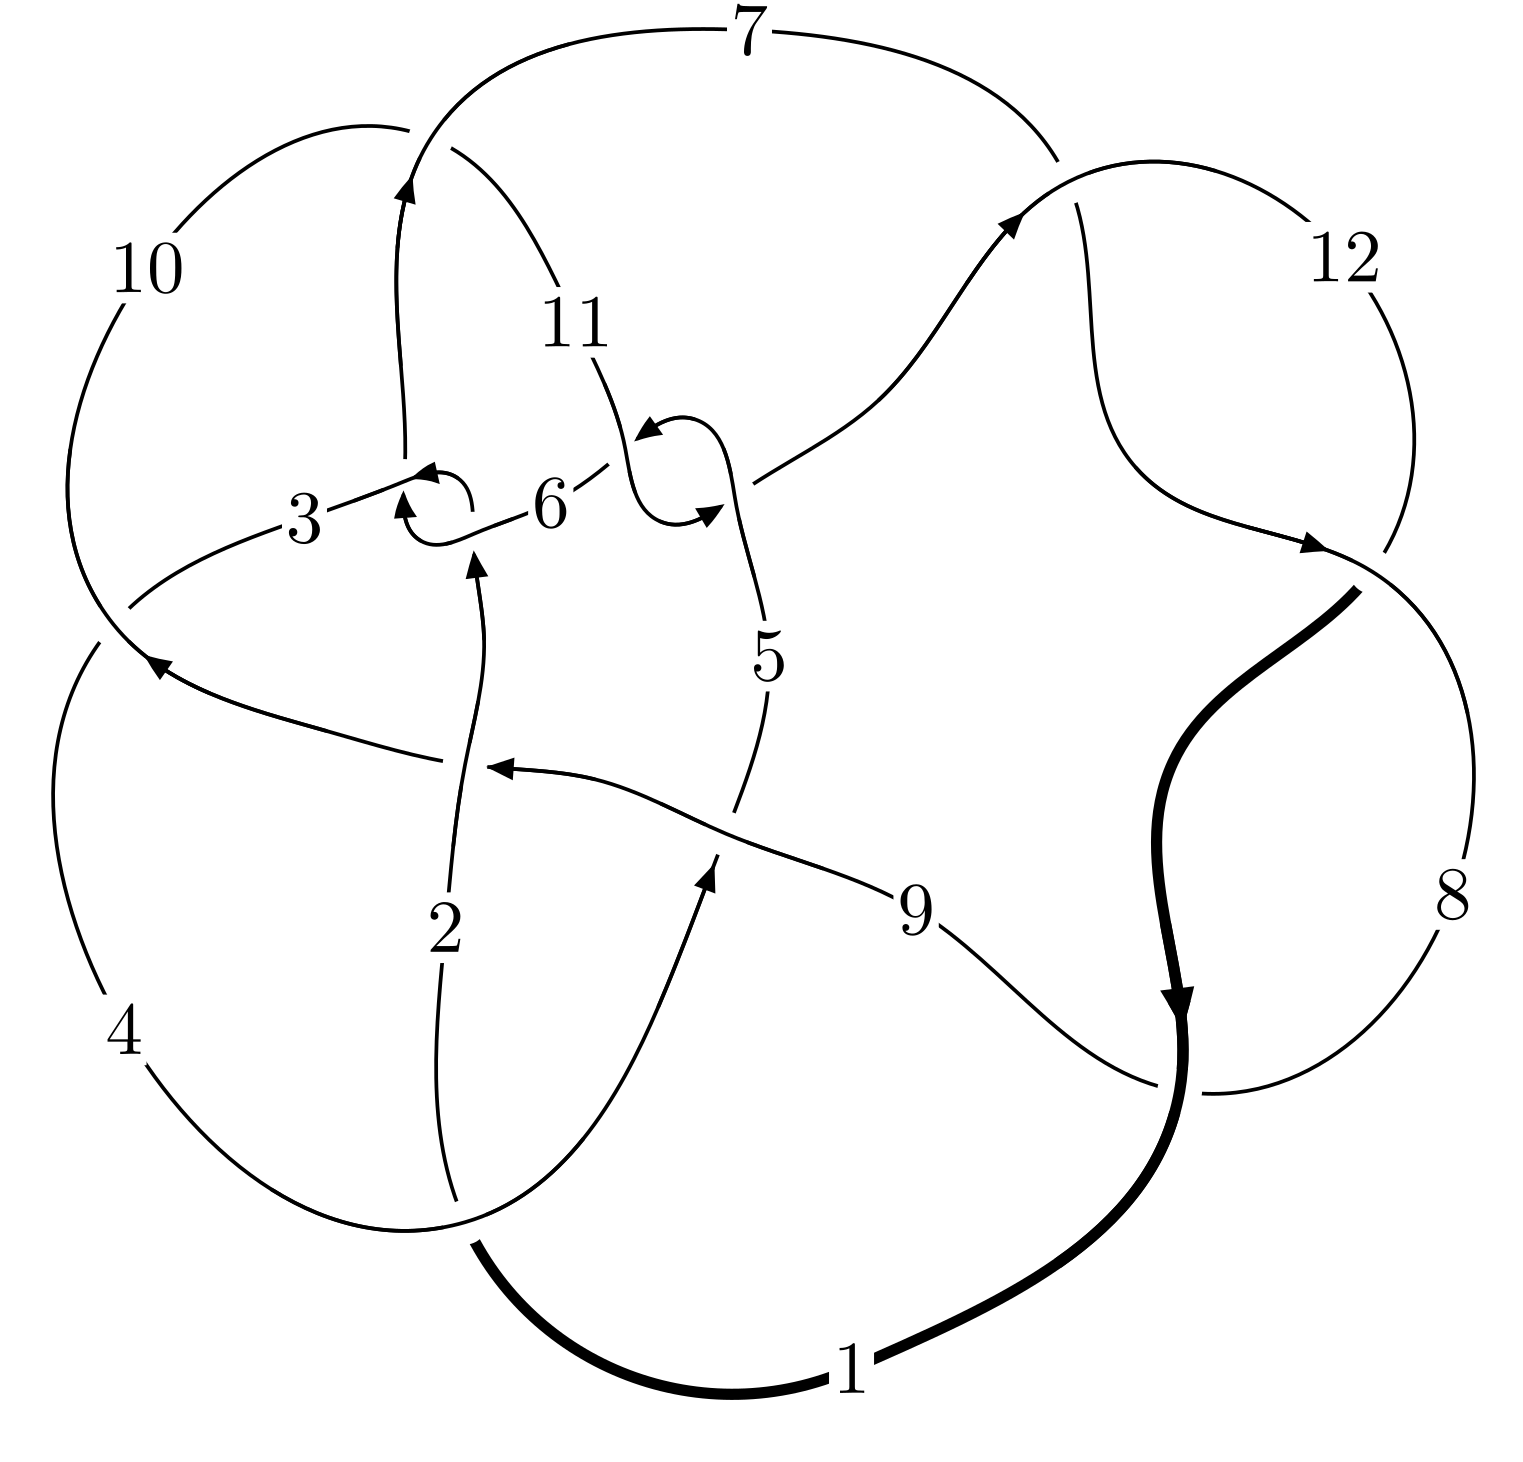
\includegraphics[width=112pt]{../../../GIT/diagram.site/Diagrams/png/1757_12a_0956.png}\\
\ \ \ A knot diagram\footnotemark}&
\allowdisplaybreaks
\textbf{Linearized knot diagam} \\
\cline{2-2}
 &
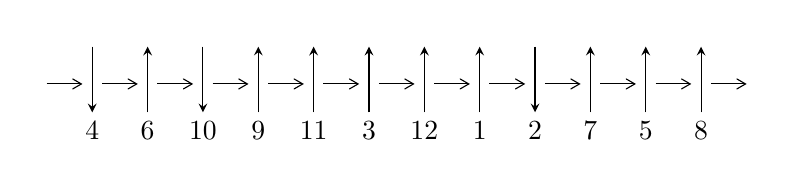
\begin{tikzpicture}[x=20pt, y=17pt]
	% nodes
	\node (C0) at (0, 0) {};
	\node (C1) at (1, 0) {};
	\node (C1U) at (1, +1) {};
	\node (C1D) at (1, -1) {4};

	\node (C2) at (2, 0) {};
	\node (C2U) at (2, +1) {};
	\node (C2D) at (2, -1) {6};

	\node (C3) at (3, 0) {};
	\node (C3U) at (3, +1) {};
	\node (C3D) at (3, -1) {10};

	\node (C4) at (4, 0) {};
	\node (C4U) at (4, +1) {};
	\node (C4D) at (4, -1) {9};

	\node (C5) at (5, 0) {};
	\node (C5U) at (5, +1) {};
	\node (C5D) at (5, -1) {11};

	\node (C6) at (6, 0) {};
	\node (C6U) at (6, +1) {};
	\node (C6D) at (6, -1) {3};

	\node (C7) at (7, 0) {};
	\node (C7U) at (7, +1) {};
	\node (C7D) at (7, -1) {12};

	\node (C8) at (8, 0) {};
	\node (C8U) at (8, +1) {};
	\node (C8D) at (8, -1) {1};

	\node (C9) at (9, 0) {};
	\node (C9U) at (9, +1) {};
	\node (C9D) at (9, -1) {2};

	\node (C10) at (10, 0) {};
	\node (C10U) at (10, +1) {};
	\node (C10D) at (10, -1) {7};

	\node (C11) at (11, 0) {};
	\node (C11U) at (11, +1) {};
	\node (C11D) at (11, -1) {5};

	\node (C12) at (12, 0) {};
	\node (C12U) at (12, +1) {};
	\node (C12D) at (12, -1) {8};
	\node (C13) at (13, 0) {};

	% arrows
	\draw[->,>={angle 60}]
	(C0) edge (C1) (C1) edge (C2) (C2) edge (C3) (C3) edge (C4) (C4) edge (C5) (C5) edge (C6) (C6) edge (C7) (C7) edge (C8) (C8) edge (C9) (C9) edge (C10) (C10) edge (C11) (C11) edge (C12) (C12) edge (C13) ;	\draw[->,>=stealth]
	(C1U) edge (C1D) (C2D) edge (C2U) (C3U) edge (C3D) (C4D) edge (C4U) (C5D) edge (C5U) (C6D) edge (C6U) (C7D) edge (C7U) (C8D) edge (C8U) (C9U) edge (C9D) (C10D) edge (C10U) (C11D) edge (C11U) (C12D) edge (C12U) ;
	\end{tikzpicture} \\
\hhline{~~} \\& 
\textbf{Solving Sequence} \\ \cline{2-2} 
 &
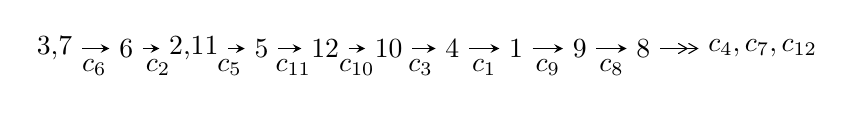
\begin{tikzpicture}[x=23pt, y=7pt]
	% node
	\node (A0) at (-1/8, 0) {3,7};
	\node (A1) at (1, 0) {6};
	\node (A2) at (33/16, 0) {2,11};
	\node (A3) at (25/8, 0) {5};
	\node (A4) at (33/8, 0) {12};
	\node (A5) at (41/8, 0) {10};
	\node (A6) at (49/8, 0) {4};
	\node (A7) at (57/8, 0) {1};
	\node (A8) at (65/8, 0) {9};
	\node (A9) at (73/8, 0) {8};
	\node (C1) at (1/2, -1) {$c_{6}$};
	\node (C2) at (3/2, -1) {$c_{2}$};
	\node (C3) at (21/8, -1) {$c_{5}$};
	\node (C4) at (29/8, -1) {$c_{11}$};
	\node (C5) at (37/8, -1) {$c_{10}$};
	\node (C6) at (45/8, -1) {$c_{3}$};
	\node (C7) at (53/8, -1) {$c_{1}$};
	\node (C8) at (61/8, -1) {$c_{9}$};
	\node (C9) at (69/8, -1) {$c_{8}$};
	\node (A10) at (11, 0) {$c_{4},c_{7},c_{12}$};

	% edge
	\draw[->,>=stealth]	
	(A0) edge (A1) (A1) edge (A2) (A2) edge (A3) (A3) edge (A4) (A4) edge (A5) (A5) edge (A6) (A6) edge (A7) (A7) edge (A8) (A8) edge (A9) ;
	\draw[->>,>={angle 60}]	
	(A9) edge (A10);
\end{tikzpicture} \\ 

\end{tabular} \\

\footnotetext{
The image of knot diagram is generated by the software ``\textbf{Draw programme}" developed by Andrew Bartholomew(\url{http://www.layer8.co.uk/maths/draw/index.htm\#Running-draw}), where we modified some parts for our purpose(\url{https://github.com/CATsTAILs/LinksPainter}).
}\phantom \\ \newline 
\centering \textbf{Ideals for irreducible components\footnotemark of $X_{\text{par}}$} 
 
\begin{align*}
I^u_{1}&=\langle 
5.01989\times10^{429} u^{132}+6.06464\times10^{430} u^{131}+\cdots+3.60673\times10^{430} b+3.79307\times10^{433},\\
\phantom{I^u_{1}}&\phantom{= \langle  }6.26086\times10^{434} u^{132}+7.00442\times10^{434} u^{131}+\cdots+2.74472\times10^{433} a-3.98484\times10^{437},\\
\phantom{I^u_{1}}&\phantom{= \langle  }u^{133}-35 u^{131}+\cdots-192 u+761\rangle \\
I^u_{2}&=\langle 
305069750 u^{28}+681402822 u^{27}+\cdots+8159603 b-631763705,\\
\phantom{I^u_{2}}&\phantom{= \langle  }-684332979 u^{28}-1764814437 u^{27}+\cdots+8159603 a+920265249,\;u^{29}+3 u^{28}+\cdots-6 u-1\rangle \\
\\
\end{align*}
\raggedright * 2 irreducible components of $\dim_{\mathbb{C}}=0$, with total 162 representations.\\
\footnotetext{All coefficients of polynomials are rational numbers. But the coefficients are sometimes approximated in decimal forms when there is not enough margin.}
\newpage
\renewcommand{\arraystretch}{1}
\centering \section*{I. $I^u_{1}= \langle 5.02\times10^{429} u^{132}+6.06\times10^{430} u^{131}+\cdots+3.61\times10^{430} b+3.79\times10^{433},\;6.26\times10^{434} u^{132}+7.00\times10^{434} u^{131}+\cdots+2.74\times10^{433} a-3.98\times10^{437},\;u^{133}-35 u^{131}+\cdots-192 u+761 \rangle$}
\flushleft \textbf{(i) Arc colorings}\\
\begin{tabular}{m{7pt} m{180pt} m{7pt} m{180pt} }
\flushright $a_{3}=$&$\begin{pmatrix}0\\u\end{pmatrix}$ \\
\flushright $a_{7}=$&$\begin{pmatrix}1\\0\end{pmatrix}$ \\
\flushright $a_{6}=$&$\begin{pmatrix}1\\u^2\end{pmatrix}$ \\
\flushright $a_{2}=$&$\begin{pmatrix}- u\\- u^3+u\end{pmatrix}$ \\
\flushright $a_{11}=$&$\begin{pmatrix}-22.8106 u^{132}-25.5196 u^{131}+\cdots+7406.48 u+14518.2\\-0.139181 u^{132}-1.68148 u^{131}+\cdots-1709.02 u-1051.67\end{pmatrix}$ \\
\flushright $a_{5}=$&$\begin{pmatrix}-18.6049 u^{132}-9.07059 u^{131}+\cdots+21422.0 u+20981.3\\-1.74155 u^{132}+6.42924 u^{131}+\cdots+14068.1 u+8478.97\end{pmatrix}$ \\
\flushright $a_{12}=$&$\begin{pmatrix}-258.222 u^{132}-229.030 u^{131}+\cdots+193487. u+221526.\\2.69839 u^{132}+1.79774 u^{131}+\cdots-2931.78 u-2819.29\end{pmatrix}$ \\
\flushright $a_{10}=$&$\begin{pmatrix}-22.6714 u^{132}-23.8382 u^{131}+\cdots+9115.50 u+15569.9\\-0.139181 u^{132}-1.68148 u^{131}+\cdots-1709.02 u-1051.67\end{pmatrix}$ \\
\flushright $a_{4}=$&$\begin{pmatrix}-16.9499 u^{132}-17.0235 u^{131}+\cdots+4983.99 u+11235.4\\2.54388 u^{132}+2.52094 u^{131}+\cdots-1084.16 u-1796.53\end{pmatrix}$ \\
\flushright $a_{1}=$&$\begin{pmatrix}-151.474 u^{132}-154.130 u^{131}+\cdots+82798.9 u+113115.\\10.4126 u^{132}+9.97071 u^{131}+\cdots-5024.52 u-7744.52\end{pmatrix}$ \\
\flushright $a_{9}=$&$\begin{pmatrix}-27.4107 u^{132}-30.6810 u^{131}+\cdots+7765.47 u+17086.0\\-3.58075 u^{132}-3.60481 u^{131}+\cdots+1933.82 u+2639.59\end{pmatrix}$ \\
\flushright $a_{8}=$&$\begin{pmatrix}306.838 u^{132}+285.363 u^{131}+\cdots-208577. u-251784.\\-11.8525 u^{132}-10.7196 u^{131}+\cdots+6720.53 u+9349.95\end{pmatrix}$\\&\end{tabular}
\flushleft \textbf{(ii) Obstruction class $= -1$}\\~\\
\flushleft \textbf{(iii) Cusp Shapes $= 237.869 u^{132}+195.350 u^{131}+\cdots-206753. u-218314.$}\\~\\
\newpage\renewcommand{\arraystretch}{1}
\flushleft \textbf{(iv) u-Polynomials at the component}\newline \\
\begin{tabular}{m{50pt}|m{274pt}}
Crossings & \hspace{64pt}u-Polynomials at each crossing \\
\hline $$\begin{aligned}c_{1}\end{aligned}$$&$\begin{aligned}
&u^{133}-5 u^{132}+\cdots-161632 u-14048
\end{aligned}$\\
\hline $$\begin{aligned}c_{2},c_{6}\end{aligned}$$&$\begin{aligned}
&u^{133}-35 u^{131}+\cdots-192 u+761
\end{aligned}$\\
\hline $$\begin{aligned}c_{3}\end{aligned}$$&$\begin{aligned}
&u^{133}- u^{132}+\cdots-4726716 u-515789
\end{aligned}$\\
\hline $$\begin{aligned}c_{4}\end{aligned}$$&$\begin{aligned}
&u^{133}+3 u^{132}+\cdots+41074 u+6061
\end{aligned}$\\
\hline $$\begin{aligned}c_{5},c_{11}\end{aligned}$$&$\begin{aligned}
&u^{133}- u^{132}+\cdots-45568 u-71168
\end{aligned}$\\
\hline $$\begin{aligned}c_{7},c_{8},c_{12}\end{aligned}$$&$\begin{aligned}
&u^{133}+u^{132}+\cdots-20 u-1
\end{aligned}$\\
\hline $$\begin{aligned}c_{9}\end{aligned}$$&$\begin{aligned}
&u^{133}- u^{132}+\cdots-546 u-43
\end{aligned}$\\
\hline $$\begin{aligned}c_{10}\end{aligned}$$&$\begin{aligned}
&u^{133}-2 u^{132}+\cdots-540770 u+77627
\end{aligned}$\\
\hline
\end{tabular}\\~\\
\newpage\renewcommand{\arraystretch}{1}
\flushleft \textbf{(v) Riley Polynomials at the component}\newline \\
\begin{tabular}{m{50pt}|m{274pt}}
Crossings & \hspace{64pt}Riley Polynomials at each crossing \\
\hline $$\begin{aligned}c_{1}\end{aligned}$$&$\begin{aligned}
&y^{133}+11 y^{132}+\cdots+71281468928 y-197346304
\end{aligned}$\\
\hline $$\begin{aligned}c_{2},c_{6}\end{aligned}$$&$\begin{aligned}
&y^{133}-70 y^{132}+\cdots+16482074 y-579121
\end{aligned}$\\
\hline $$\begin{aligned}c_{3}\end{aligned}$$&$\begin{aligned}
&y^{133}+9 y^{132}+\cdots+782897585812 y-266038292521
\end{aligned}$\\
\hline $$\begin{aligned}c_{4}\end{aligned}$$&$\begin{aligned}
&y^{133}-13 y^{132}+\cdots-508705604 y-36735721
\end{aligned}$\\
\hline $$\begin{aligned}c_{5},c_{11}\end{aligned}$$&$\begin{aligned}
&y^{133}+49 y^{132}+\cdots-137462939648 y-5064884224
\end{aligned}$\\
\hline $$\begin{aligned}c_{7},c_{8},c_{12}\end{aligned}$$&$\begin{aligned}
&y^{133}-135 y^{132}+\cdots+164 y-1
\end{aligned}$\\
\hline $$\begin{aligned}c_{9}\end{aligned}$$&$\begin{aligned}
&y^{133}-17 y^{132}+\cdots+624486 y-1849
\end{aligned}$\\
\hline $$\begin{aligned}c_{10}\end{aligned}$$&$\begin{aligned}
&y^{133}-34 y^{132}+\cdots+514331922226 y-6025951129
\end{aligned}$\\
\hline
\end{tabular}\\~\\
\newpage\flushleft \textbf{(vi) Complex Volumes and Cusp Shapes}
$$\begin{array}{c|c|c}  
\text{Solutions to }I^u_{1}& \I (\text{vol} + \sqrt{-1}CS) & \text{Cusp shape}\\
 \hline 
\begin{aligned}
u &= \phantom{-}0.988920 + 0.138600 I \\
a &= -0.01868 + 2.61482 I \\
b &= \phantom{-}0.111075 - 0.454031 I\end{aligned}
 & \phantom{-}5.06561 + 0.42762 I & \phantom{-0.000000 } 0 \\ \hline\begin{aligned}
u &= \phantom{-}0.988920 - 0.138600 I \\
a &= -0.01868 - 2.61482 I \\
b &= \phantom{-}0.111075 + 0.454031 I\end{aligned}
 & \phantom{-}5.06561 - 0.42762 I & \phantom{-0.000000 } 0 \\ \hline\begin{aligned}
u &= -0.873966 + 0.444822 I \\
a &= \phantom{-}1.83735 - 0.05270 I \\
b &= \phantom{-}0.797900 - 0.326681 I\end{aligned}
 & -3.07390 - 2.52617 I & \phantom{-0.000000 } 0 \\ \hline\begin{aligned}
u &= -0.873966 - 0.444822 I \\
a &= \phantom{-}1.83735 + 0.05270 I \\
b &= \phantom{-}0.797900 + 0.326681 I\end{aligned}
 & -3.07390 + 2.52617 I & \phantom{-0.000000 } 0 \\ \hline\begin{aligned}
u &= -0.934196 + 0.415806 I \\
a &= -2.09634 + 0.44286 I \\
b &= -0.578069 + 0.732095 I\end{aligned}
 & -3.01255 - 6.47573 I & \phantom{-0.000000 } 0 \\ \hline\begin{aligned}
u &= -0.934196 - 0.415806 I \\
a &= -2.09634 - 0.44286 I \\
b &= -0.578069 - 0.732095 I\end{aligned}
 & -3.01255 + 6.47573 I & \phantom{-0.000000 } 0 \\ \hline\begin{aligned}
u &= -0.944903 + 0.394113 I \\
a &= \phantom{-}2.37299 - 0.55951 I \\
b &= \phantom{-}0.512928 - 0.998907 I\end{aligned}
 & \phantom{-}3.62121 - 9.53053 I & \phantom{-0.000000 } 0 \\ \hline\begin{aligned}
u &= -0.944903 - 0.394113 I \\
a &= \phantom{-}2.37299 + 0.55951 I \\
b &= \phantom{-}0.512928 + 0.998907 I\end{aligned}
 & \phantom{-}3.62121 + 9.53053 I & \phantom{-0.000000 } 0 \\ \hline\begin{aligned}
u &= \phantom{-}0.931719\phantom{ +0.000000I} \\
a &= \phantom{-}7.28657\phantom{ +0.000000I} \\
b &= \phantom{-}0.174112\phantom{ +0.000000I}\end{aligned}
 & \phantom{-}4.76527\phantom{ +0.000000I} & \phantom{-0.000000 } 0 \\ \hline\begin{aligned}
u &= \phantom{-}0.908709 + 0.198506 I \\
a &= -1.49042 + 0.12597 I \\
b &= -1.16136 + 1.05086 I\end{aligned}
 & -1.15100 + 1.00525 I & \phantom{-0.000000 } 0\\
 \hline 
 \end{array}$$\newpage$$\begin{array}{c|c|c}  
\text{Solutions to }I^u_{1}& \I (\text{vol} + \sqrt{-1}CS) & \text{Cusp shape}\\
 \hline 
\begin{aligned}
u &= \phantom{-}0.908709 - 0.198506 I \\
a &= -1.49042 - 0.12597 I \\
b &= -1.16136 - 1.05086 I\end{aligned}
 & -1.15100 - 1.00525 I & \phantom{-0.000000 } 0 \\ \hline\begin{aligned}
u &= -0.775714 + 0.512116 I \\
a &= \phantom{-}1.36243 + 0.77522 I \\
b &= \phantom{-}1.063830 + 0.532036 I\end{aligned}
 & -3.35517 - 2.09583 I & \phantom{-0.000000 } 0 \\ \hline\begin{aligned}
u &= -0.775714 - 0.512116 I \\
a &= \phantom{-}1.36243 - 0.77522 I \\
b &= \phantom{-}1.063830 - 0.532036 I\end{aligned}
 & -3.35517 + 2.09583 I & \phantom{-0.000000 } 0 \\ \hline\begin{aligned}
u &= -0.173448 + 1.057700 I \\
a &= -0.118423 - 0.201854 I \\
b &= -0.628440 - 0.802795 I\end{aligned}
 & \phantom{-}0.26270 + 4.87247 I & \phantom{-0.000000 } 0 \\ \hline\begin{aligned}
u &= -0.173448 - 1.057700 I \\
a &= -0.118423 + 0.201854 I \\
b &= -0.628440 + 0.802795 I\end{aligned}
 & \phantom{-}0.26270 - 4.87247 I & \phantom{-0.000000 } 0 \\ \hline\begin{aligned}
u &= -0.761394 + 0.524998 I \\
a &= -1.71016 - 1.20594 I \\
b &= -1.59048 - 0.60273 I\end{aligned}
 & \phantom{-}0.85958 - 2.13851 I & \phantom{-0.000000 } 0 \\ \hline\begin{aligned}
u &= -0.761394 - 0.524998 I \\
a &= -1.71016 + 1.20594 I \\
b &= -1.59048 + 0.60273 I\end{aligned}
 & \phantom{-}0.85958 + 2.13851 I & \phantom{-0.000000 } 0 \\ \hline\begin{aligned}
u &= \phantom{-}0.854372 + 0.353578 I \\
a &= -2.58243 - 1.22405 I \\
b &= -1.02493 - 1.47052 I\end{aligned}
 & \phantom{-}3.73823 - 5.31287 I & \phantom{-0.000000 } 0 \\ \hline\begin{aligned}
u &= \phantom{-}0.854372 - 0.353578 I \\
a &= -2.58243 + 1.22405 I \\
b &= -1.02493 + 1.47052 I\end{aligned}
 & \phantom{-}3.73823 + 5.31287 I & \phantom{-0.000000 } 0 \\ \hline\begin{aligned}
u &= \phantom{-}0.901145 + 0.204526 I \\
a &= -2.19001 - 0.49699 I \\
b &= -1.287730 + 0.221407 I\end{aligned}
 & -1.15876 + 0.86950 I & \phantom{-0.000000 } 0\\
 \hline 
 \end{array}$$\newpage$$\begin{array}{c|c|c}  
\text{Solutions to }I^u_{1}& \I (\text{vol} + \sqrt{-1}CS) & \text{Cusp shape}\\
 \hline 
\begin{aligned}
u &= \phantom{-}0.901145 - 0.204526 I \\
a &= -2.19001 + 0.49699 I \\
b &= -1.287730 - 0.221407 I\end{aligned}
 & -1.15876 - 0.86950 I & \phantom{-0.000000 } 0 \\ \hline\begin{aligned}
u &= \phantom{-}0.865077 + 0.291875 I \\
a &= \phantom{-}2.54001 + 0.96713 I \\
b &= \phantom{-}1.14692 + 0.91206 I\end{aligned}
 & -2.30330 - 2.38565 I & \phantom{-0.000000 } 0 \\ \hline\begin{aligned}
u &= \phantom{-}0.865077 - 0.291875 I \\
a &= \phantom{-}2.54001 - 0.96713 I \\
b &= \phantom{-}1.14692 - 0.91206 I\end{aligned}
 & -2.30330 + 2.38565 I & \phantom{-0.000000 } 0 \\ \hline\begin{aligned}
u &= \phantom{-}0.029311 + 0.911005 I \\
a &= -0.071683 + 0.543041 I \\
b &= -1.068210 - 0.220558 I\end{aligned}
 & \phantom{-}7.28500 + 6.69681 I & \phantom{-0.000000 } 0 \\ \hline\begin{aligned}
u &= \phantom{-}0.029311 - 0.911005 I \\
a &= -0.071683 - 0.543041 I \\
b &= -1.068210 + 0.220558 I\end{aligned}
 & \phantom{-}7.28500 - 6.69681 I & \phantom{-0.000000 } 0 \\ \hline\begin{aligned}
u &= -0.198853 + 0.888063 I \\
a &= -0.494799 - 0.516999 I \\
b &= \phantom{-}0.605104 - 0.646999 I\end{aligned}
 & \phantom{-}4.45599 - 5.34269 I & \phantom{-0.000000 } 0 \\ \hline\begin{aligned}
u &= -0.198853 - 0.888063 I \\
a &= -0.494799 + 0.516999 I \\
b &= \phantom{-}0.605104 + 0.646999 I\end{aligned}
 & \phantom{-}4.45599 + 5.34269 I & \phantom{-0.000000 } 0 \\ \hline\begin{aligned}
u &= -0.783519 + 0.445304 I \\
a &= -0.520026 - 1.227660 I \\
b &= -0.76729 - 1.28515 I\end{aligned}
 & \phantom{-}2.37891 - 3.23849 I & \phantom{-0.000000 } 0 \\ \hline\begin{aligned}
u &= -0.783519 - 0.445304 I \\
a &= -0.520026 + 1.227660 I \\
b &= -0.76729 + 1.28515 I\end{aligned}
 & \phantom{-}2.37891 + 3.23849 I & \phantom{-0.000000 } 0 \\ \hline\begin{aligned}
u &= \phantom{-}1.092180 + 0.150295 I \\
a &= -1.182540 - 0.068170 I \\
b &= -0.069476 - 0.254256 I\end{aligned}
 & \phantom{-}6.52211 - 0.06200 I & \phantom{-0.000000 } 0\\
 \hline 
 \end{array}$$\newpage$$\begin{array}{c|c|c}  
\text{Solutions to }I^u_{1}& \I (\text{vol} + \sqrt{-1}CS) & \text{Cusp shape}\\
 \hline 
\begin{aligned}
u &= \phantom{-}1.092180 - 0.150295 I \\
a &= -1.182540 + 0.068170 I \\
b &= -0.069476 + 0.254256 I\end{aligned}
 & \phantom{-}6.52211 + 0.06200 I & \phantom{-0.000000 } 0 \\ \hline\begin{aligned}
u &= \phantom{-}0.862696 + 0.233785 I \\
a &= \phantom{-}0.262514 - 1.252500 I \\
b &= \phantom{-}0.62670 - 2.07541 I\end{aligned}
 & -2.43076 + 4.82491 I & \phantom{-0.000000 } 0 \\ \hline\begin{aligned}
u &= \phantom{-}0.862696 - 0.233785 I \\
a &= \phantom{-}0.262514 + 1.252500 I \\
b &= \phantom{-}0.62670 + 2.07541 I\end{aligned}
 & -2.43076 - 4.82491 I & \phantom{-0.000000 } 0 \\ \hline\begin{aligned}
u &= \phantom{-}0.028491 + 0.886624 I \\
a &= -0.074201 - 0.428514 I \\
b &= \phantom{-}0.738909 + 0.306732 I\end{aligned}
 & \phantom{-}0.50495 + 4.20405 I & \phantom{-0.000000 } 0 \\ \hline\begin{aligned}
u &= \phantom{-}0.028491 - 0.886624 I \\
a &= -0.074201 + 0.428514 I \\
b &= \phantom{-}0.738909 - 0.306732 I\end{aligned}
 & \phantom{-}0.50495 - 4.20405 I & \phantom{-0.000000 } 0 \\ \hline\begin{aligned}
u &= -0.932420 + 0.620236 I \\
a &= \phantom{-}1.30938 + 1.41471 I \\
b &= \phantom{-}2.11417 - 0.03152 I\end{aligned}
 & \phantom{-}9.81908 - 2.45914 I & \phantom{-0.000000 } 0 \\ \hline\begin{aligned}
u &= -0.932420 - 0.620236 I \\
a &= \phantom{-}1.30938 - 1.41471 I \\
b &= \phantom{-}2.11417 + 0.03152 I\end{aligned}
 & \phantom{-}9.81908 + 2.45914 I & \phantom{-0.000000 } 0 \\ \hline\begin{aligned}
u &= \phantom{-}0.285616 + 1.083460 I \\
a &= \phantom{-}0.110519 + 0.446575 I \\
b &= -1.030560 + 0.863341 I\end{aligned}
 & \phantom{-}4.00112 - 12.85700 I & \phantom{-0.000000 } 0 \\ \hline\begin{aligned}
u &= \phantom{-}0.285616 - 1.083460 I \\
a &= \phantom{-}0.110519 - 0.446575 I \\
b &= -1.030560 - 0.863341 I\end{aligned}
 & \phantom{-}4.00112 + 12.85700 I & \phantom{-0.000000 } 0 \\ \hline\begin{aligned}
u &= \phantom{-}1.065690 + 0.366918 I \\
a &= -1.120320 + 0.685903 I \\
b &= -0.938404 - 0.798931 I\end{aligned}
 & \phantom{-}3.10610 + 2.82928 I & \phantom{-0.000000 } 0\\
 \hline 
 \end{array}$$\newpage$$\begin{array}{c|c|c}  
\text{Solutions to }I^u_{1}& \I (\text{vol} + \sqrt{-1}CS) & \text{Cusp shape}\\
 \hline 
\begin{aligned}
u &= \phantom{-}1.065690 - 0.366918 I \\
a &= -1.120320 - 0.685903 I \\
b &= -0.938404 + 0.798931 I\end{aligned}
 & \phantom{-}3.10610 - 2.82928 I & \phantom{-0.000000 } 0 \\ \hline\begin{aligned}
u &= \phantom{-}0.826927 + 0.279525 I \\
a &= \phantom{-}0.51622 + 1.59722 I \\
b &= -0.22930 + 2.40332 I\end{aligned}
 & \phantom{-}3.53976 + 8.18292 I & \phantom{-0.000000 } 0 \\ \hline\begin{aligned}
u &= \phantom{-}0.826927 - 0.279525 I \\
a &= \phantom{-}0.51622 - 1.59722 I \\
b &= -0.22930 - 2.40332 I\end{aligned}
 & \phantom{-}3.53976 - 8.18292 I & \phantom{-0.000000 } 0 \\ \hline\begin{aligned}
u &= -0.424218 + 1.049990 I \\
a &= \phantom{-}0.113537 + 0.393271 I \\
b &= \phantom{-}0.690952 + 0.630816 I\end{aligned}
 & -3.97298 + 1.45301 I & \phantom{-0.000000 } 0 \\ \hline\begin{aligned}
u &= -0.424218 - 1.049990 I \\
a &= \phantom{-}0.113537 - 0.393271 I \\
b &= \phantom{-}0.690952 - 0.630816 I\end{aligned}
 & -3.97298 - 1.45301 I & \phantom{-0.000000 } 0 \\ \hline\begin{aligned}
u &= \phantom{-}0.851786\phantom{ +0.000000I} \\
a &= -3.75611\phantom{ +0.000000I} \\
b &= -0.269450\phantom{ +0.000000I}\end{aligned}
 & -0.410389\phantom{ +0.000000I} & \phantom{-0.000000 } 0 \\ \hline\begin{aligned}
u &= \phantom{-}1.062380 + 0.455149 I \\
a &= \phantom{-}1.41470 - 0.98400 I \\
b &= \phantom{-}1.51030 + 0.79163 I\end{aligned}
 & \phantom{-}10.42620 + 3.06381 I & \phantom{-0.000000 } 0 \\ \hline\begin{aligned}
u &= \phantom{-}1.062380 - 0.455149 I \\
a &= \phantom{-}1.41470 + 0.98400 I \\
b &= \phantom{-}1.51030 - 0.79163 I\end{aligned}
 & \phantom{-}10.42620 - 3.06381 I & \phantom{-0.000000 } 0 \\ \hline\begin{aligned}
u &= \phantom{-}1.131830 + 0.267629 I \\
a &= \phantom{-}1.033760 - 0.530042 I \\
b &= \phantom{-}0.487134 + 0.483951 I\end{aligned}
 & \phantom{-}1.76196 + 1.04851 I & \phantom{-0.000000 } 0 \\ \hline\begin{aligned}
u &= \phantom{-}1.131830 - 0.267629 I \\
a &= \phantom{-}1.033760 + 0.530042 I \\
b &= \phantom{-}0.487134 - 0.483951 I\end{aligned}
 & \phantom{-}1.76196 - 1.04851 I & \phantom{-0.000000 } 0\\
 \hline 
 \end{array}$$\newpage$$\begin{array}{c|c|c}  
\text{Solutions to }I^u_{1}& \I (\text{vol} + \sqrt{-1}CS) & \text{Cusp shape}\\
 \hline 
\begin{aligned}
u &= \phantom{-}0.334083 + 1.131750 I \\
a &= -0.109028 - 0.451487 I \\
b &= \phantom{-}0.901936 - 0.734964 I\end{aligned}
 & -2.79092 - 8.26077 I & \phantom{-0.000000 } 0 \\ \hline\begin{aligned}
u &= \phantom{-}0.334083 - 1.131750 I \\
a &= -0.109028 + 0.451487 I \\
b &= \phantom{-}0.901936 + 0.734964 I\end{aligned}
 & -2.79092 + 8.26077 I & \phantom{-0.000000 } 0 \\ \hline\begin{aligned}
u &= -0.762042 + 0.292320 I \\
a &= -2.35692 - 0.21609 I \\
b &= -1.37735 + 0.37759 I\end{aligned}
 & \phantom{-}2.18942 - 0.22647 I & \phantom{-0.000000 } 0 \\ \hline\begin{aligned}
u &= -0.762042 - 0.292320 I \\
a &= -2.35692 + 0.21609 I \\
b &= -1.37735 - 0.37759 I\end{aligned}
 & \phantom{-}2.18942 + 0.22647 I & \phantom{-0.000000 } 0 \\ \hline\begin{aligned}
u &= -0.608932 + 0.538700 I \\
a &= \phantom{-}0.449845 + 0.286768 I \\
b &= \phantom{-}0.261800 + 1.016030 I\end{aligned}
 & -3.80544 - 1.47323 I & \phantom{-0.000000 } 0 \\ \hline\begin{aligned}
u &= -0.608932 - 0.538700 I \\
a &= \phantom{-}0.449845 - 0.286768 I \\
b &= \phantom{-}0.261800 - 1.016030 I\end{aligned}
 & -3.80544 + 1.47323 I & \phantom{-0.000000 } 0 \\ \hline\begin{aligned}
u &= \phantom{-}1.143600 + 0.376238 I \\
a &= \phantom{-}0.273466 - 1.191650 I \\
b &= \phantom{-}0.927929 - 0.091326 I\end{aligned}
 & \phantom{-}8.36637 + 0.11927 I & \phantom{-0.000000 } 0 \\ \hline\begin{aligned}
u &= \phantom{-}1.143600 - 0.376238 I \\
a &= \phantom{-}0.273466 + 1.191650 I \\
b &= \phantom{-}0.927929 + 0.091326 I\end{aligned}
 & \phantom{-}8.36637 - 0.11927 I & \phantom{-0.000000 } 0 \\ \hline\begin{aligned}
u &= \phantom{-}1.139400 + 0.398073 I \\
a &= -0.390173 + 0.667856 I \\
b &= -0.729204 - 0.149396 I\end{aligned}
 & \phantom{-}2.78580 + 1.00430 I & \phantom{-0.000000 } 0 \\ \hline\begin{aligned}
u &= \phantom{-}1.139400 - 0.398073 I \\
a &= -0.390173 - 0.667856 I \\
b &= -0.729204 + 0.149396 I\end{aligned}
 & \phantom{-}2.78580 - 1.00430 I & \phantom{-0.000000 } 0\\
 \hline 
 \end{array}$$\newpage$$\begin{array}{c|c|c}  
\text{Solutions to }I^u_{1}& \I (\text{vol} + \sqrt{-1}CS) & \text{Cusp shape}\\
 \hline 
\begin{aligned}
u &= -0.002540 + 1.220210 I \\
a &= \phantom{-}0.197241 + 0.383474 I \\
b &= -0.440573 + 0.317848 I\end{aligned}
 & -1.93173 + 0.03663 I & \phantom{-0.000000 } 0 \\ \hline\begin{aligned}
u &= -0.002540 - 1.220210 I \\
a &= \phantom{-}0.197241 - 0.383474 I \\
b &= -0.440573 - 0.317848 I\end{aligned}
 & -1.93173 - 0.03663 I & \phantom{-0.000000 } 0 \\ \hline\begin{aligned}
u &= -1.214360 + 0.136317 I \\
a &= -1.204420 - 0.050221 I \\
b &= -1.122410 + 0.673110 I\end{aligned}
 & \phantom{-}4.97319 - 1.06275 I & \phantom{-0.000000 } 0 \\ \hline\begin{aligned}
u &= -1.214360 - 0.136317 I \\
a &= -1.204420 + 0.050221 I \\
b &= -1.122410 - 0.673110 I\end{aligned}
 & \phantom{-}4.97319 + 1.06275 I & \phantom{-0.000000 } 0 \\ \hline\begin{aligned}
u &= -1.207700 + 0.257376 I \\
a &= \phantom{-}1.57680 + 0.43641 I \\
b &= \phantom{-}1.46350 - 0.50185 I\end{aligned}
 & \phantom{-}12.51590 - 4.02680 I & \phantom{-0.000000 } 0 \\ \hline\begin{aligned}
u &= -1.207700 - 0.257376 I \\
a &= \phantom{-}1.57680 - 0.43641 I \\
b &= \phantom{-}1.46350 + 0.50185 I\end{aligned}
 & \phantom{-}12.51590 + 4.02680 I & \phantom{-0.000000 } 0 \\ \hline\begin{aligned}
u &= -0.757731 + 0.975271 I \\
a &= -0.361195 - 0.577809 I \\
b &= -0.942922 - 0.388512 I\end{aligned}
 & -0.52065 - 2.57273 I & \phantom{-0.000000 } 0 \\ \hline\begin{aligned}
u &= -0.757731 - 0.975271 I \\
a &= -0.361195 + 0.577809 I \\
b &= -0.942922 + 0.388512 I\end{aligned}
 & -0.52065 + 2.57273 I & \phantom{-0.000000 } 0 \\ \hline\begin{aligned}
u &= -1.153150 + 0.473095 I \\
a &= \phantom{-}1.51225 - 0.63978 I \\
b &= \phantom{-}0.99334 - 1.65032 I\end{aligned}
 & \phantom{-}5.69421 - 7.09203 I & \phantom{-0.000000 } 0 \\ \hline\begin{aligned}
u &= -1.153150 - 0.473095 I \\
a &= \phantom{-}1.51225 + 0.63978 I \\
b &= \phantom{-}0.99334 + 1.65032 I\end{aligned}
 & \phantom{-}5.69421 + 7.09203 I & \phantom{-0.000000 } 0\\
 \hline 
 \end{array}$$\newpage$$\begin{array}{c|c|c}  
\text{Solutions to }I^u_{1}& \I (\text{vol} + \sqrt{-1}CS) & \text{Cusp shape}\\
 \hline 
\begin{aligned}
u &= -0.165049 + 0.733946 I \\
a &= \phantom{-}0.636658 - 0.216868 I \\
b &= -0.604158 - 0.995471 I\end{aligned}
 & -0.90642 + 2.57878 I & \phantom{-0.000000 } 0 \\ \hline\begin{aligned}
u &= -0.165049 - 0.733946 I \\
a &= \phantom{-}0.636658 + 0.216868 I \\
b &= -0.604158 + 0.995471 I\end{aligned}
 & -0.90642 - 2.57878 I & \phantom{-0.000000 } 0 \\ \hline\begin{aligned}
u &= -0.160724 + 0.722073 I \\
a &= -0.683291 + 0.496358 I \\
b &= \phantom{-}0.89885 + 1.13433 I\end{aligned}
 & \phantom{-}4.64169 + 3.45865 I & \phantom{-0.000000 } 0 \\ \hline\begin{aligned}
u &= -0.160724 - 0.722073 I \\
a &= -0.683291 - 0.496358 I \\
b &= \phantom{-}0.89885 - 1.13433 I\end{aligned}
 & \phantom{-}4.64169 - 3.45865 I & \phantom{-0.000000 } 0 \\ \hline\begin{aligned}
u &= -1.160620 + 0.499905 I \\
a &= \phantom{-}2.17246 - 0.11710 I \\
b &= \phantom{-}1.71400 - 1.41071 I\end{aligned}
 & \phantom{-}7.52291 - 8.04572 I & \phantom{-0.000000 } 0 \\ \hline\begin{aligned}
u &= -1.160620 - 0.499905 I \\
a &= \phantom{-}2.17246 + 0.11710 I \\
b &= \phantom{-}1.71400 + 1.41071 I\end{aligned}
 & \phantom{-}7.52291 + 8.04572 I & \phantom{-0.000000 } 0 \\ \hline\begin{aligned}
u &= -0.618910 + 0.393493 I \\
a &= -0.547880 - 0.185869 I \\
b &= \phantom{-}0.31273 + 1.54182 I\end{aligned}
 & \phantom{-}2.61970 + 6.09240 I & \phantom{-0.000000 } 0 \\ \hline\begin{aligned}
u &= -0.618910 - 0.393493 I \\
a &= -0.547880 + 0.185869 I \\
b &= \phantom{-}0.31273 - 1.54182 I\end{aligned}
 & \phantom{-}2.61970 - 6.09240 I & \phantom{-0.000000 } 0 \\ \hline\begin{aligned}
u &= -1.166780 + 0.501329 I \\
a &= -1.84073 + 0.17891 I \\
b &= -1.40773 + 1.35918 I\end{aligned}
 & \phantom{-}2.00330 - 7.20728 I & \phantom{-0.000000 } 0 \\ \hline\begin{aligned}
u &= -1.166780 - 0.501329 I \\
a &= -1.84073 - 0.17891 I \\
b &= -1.40773 - 1.35918 I\end{aligned}
 & \phantom{-}2.00330 + 7.20728 I & \phantom{-0.000000 } 0\\
 \hline 
 \end{array}$$\newpage$$\begin{array}{c|c|c}  
\text{Solutions to }I^u_{1}& \I (\text{vol} + \sqrt{-1}CS) & \text{Cusp shape}\\
 \hline 
\begin{aligned}
u &= -0.579212 + 0.439699 I \\
a &= \phantom{-}0.0389490 + 0.0109292 I \\
b &= -0.275486 - 1.347110 I\end{aligned}
 & -4.04146 + 2.82999 I & \phantom{-0.000000 } 0 \\ \hline\begin{aligned}
u &= -0.579212 - 0.439699 I \\
a &= \phantom{-}0.0389490 - 0.0109292 I \\
b &= -0.275486 + 1.347110 I\end{aligned}
 & -4.04146 - 2.82999 I & \phantom{-0.000000 } 0 \\ \hline\begin{aligned}
u &= \phantom{-}0.454290 + 1.197280 I \\
a &= -0.047155 - 0.383391 I \\
b &= \phantom{-}0.174568 - 0.238990 I\end{aligned}
 & \phantom{-}1.73556 + 5.22677 I & \phantom{-0.000000 } 0 \\ \hline\begin{aligned}
u &= \phantom{-}0.454290 - 1.197280 I \\
a &= -0.047155 + 0.383391 I \\
b &= \phantom{-}0.174568 + 0.238990 I\end{aligned}
 & \phantom{-}1.73556 - 5.22677 I & \phantom{-0.000000 } 0 \\ \hline\begin{aligned}
u &= -1.106620 + 0.697966 I \\
a &= -1.272150 - 0.497172 I \\
b &= -1.37278 + 0.44356 I\end{aligned}
 & \phantom{-}0.77664 - 3.65523 I & \phantom{-0.000000 } 0 \\ \hline\begin{aligned}
u &= -1.106620 - 0.697966 I \\
a &= -1.272150 + 0.497172 I \\
b &= -1.37278 - 0.44356 I\end{aligned}
 & \phantom{-}0.77664 + 3.65523 I & \phantom{-0.000000 } 0 \\ \hline\begin{aligned}
u &= -0.184238 + 0.660636 I \\
a &= -1.234280 - 0.029458 I \\
b &= \phantom{-}0.080549 + 1.243700 I\end{aligned}
 & \phantom{-}2.89142 + 2.74667 I & \phantom{-0.000000 } 0 \\ \hline\begin{aligned}
u &= -0.184238 - 0.660636 I \\
a &= -1.234280 + 0.029458 I \\
b &= \phantom{-}0.080549 - 1.243700 I\end{aligned}
 & \phantom{-}2.89142 - 2.74667 I & \phantom{-0.000000 } 0 \\ \hline\begin{aligned}
u &= \phantom{-}1.248630 + 0.410313 I \\
a &= \phantom{-}1.81681 + 0.26127 I \\
b &= \phantom{-}1.71039 + 0.89846 I\end{aligned}
 & \phantom{-}8.74578 + 9.62632 I & \phantom{-0.000000 } 0 \\ \hline\begin{aligned}
u &= \phantom{-}1.248630 - 0.410313 I \\
a &= \phantom{-}1.81681 - 0.26127 I \\
b &= \phantom{-}1.71039 - 0.89846 I\end{aligned}
 & \phantom{-}8.74578 - 9.62632 I & \phantom{-0.000000 } 0\\
 \hline 
 \end{array}$$\newpage$$\begin{array}{c|c|c}  
\text{Solutions to }I^u_{1}& \I (\text{vol} + \sqrt{-1}CS) & \text{Cusp shape}\\
 \hline 
\begin{aligned}
u &= \phantom{-}0.247277 + 0.633247 I \\
a &= -0.731723 - 0.129482 I \\
b &= \phantom{-}1.101850 - 0.140895 I\end{aligned}
 & \phantom{-}8.19994 + 1.08329 I & \phantom{-0.000000 } 0 \\ \hline\begin{aligned}
u &= \phantom{-}0.247277 - 0.633247 I \\
a &= -0.731723 + 0.129482 I \\
b &= \phantom{-}1.101850 + 0.140895 I\end{aligned}
 & \phantom{-}8.19994 - 1.08329 I & \phantom{-0.000000 } 0 \\ \hline\begin{aligned}
u &= \phantom{-}0.495483 + 1.229530 I \\
a &= \phantom{-}0.040797 + 0.456616 I \\
b &= -0.829436 + 0.437930 I\end{aligned}
 & -2.35885 - 1.74213 I & \phantom{-0.000000 } 0 \\ \hline\begin{aligned}
u &= \phantom{-}0.495483 - 1.229530 I \\
a &= \phantom{-}0.040797 - 0.456616 I \\
b &= -0.829436 - 0.437930 I\end{aligned}
 & -2.35885 + 1.74213 I & \phantom{-0.000000 } 0 \\ \hline\begin{aligned}
u &= -1.263980 + 0.418103 I \\
a &= -0.616231 - 0.073037 I \\
b &= -0.520940 + 0.857049 I\end{aligned}
 & \phantom{-}2.85639 - 5.09763 I & \phantom{-0.000000 } 0 \\ \hline\begin{aligned}
u &= -1.263980 - 0.418103 I \\
a &= -0.616231 + 0.073037 I \\
b &= -0.520940 - 0.857049 I\end{aligned}
 & \phantom{-}2.85639 + 5.09763 I & \phantom{-0.000000 } 0 \\ \hline\begin{aligned}
u &= -1.250780 + 0.468648 I \\
a &= \phantom{-}1.169820 + 0.380734 I \\
b &= \phantom{-}0.958896 - 0.807384 I\end{aligned}
 & \phantom{-}4.33761 - 8.97687 I & \phantom{-0.000000 } 0 \\ \hline\begin{aligned}
u &= -1.250780 - 0.468648 I \\
a &= \phantom{-}1.169820 - 0.380734 I \\
b &= \phantom{-}0.958896 + 0.807384 I\end{aligned}
 & \phantom{-}4.33761 + 8.97687 I & \phantom{-0.000000 } 0 \\ \hline\begin{aligned}
u &= -1.263460 + 0.467491 I \\
a &= -1.28082 - 0.69208 I \\
b &= -1.082550 + 0.659477 I\end{aligned}
 & \phantom{-}11.2089 - 11.5392 I & \phantom{-0.000000 } 0 \\ \hline\begin{aligned}
u &= -1.263460 - 0.467491 I \\
a &= -1.28082 + 0.69208 I \\
b &= -1.082550 - 0.659477 I\end{aligned}
 & \phantom{-}11.2089 + 11.5392 I & \phantom{-0.000000 } 0\\
 \hline 
 \end{array}$$\newpage$$\begin{array}{c|c|c}  
\text{Solutions to }I^u_{1}& \I (\text{vol} + \sqrt{-1}CS) & \text{Cusp shape}\\
 \hline 
\begin{aligned}
u &= \phantom{-}1.301980 + 0.416420 I \\
a &= -1.37864 - 0.31823 I \\
b &= -1.31422 - 0.88798 I\end{aligned}
 & \phantom{-}2.78087 + 5.23361 I & \phantom{-0.000000 } 0 \\ \hline\begin{aligned}
u &= \phantom{-}1.301980 - 0.416420 I \\
a &= -1.37864 + 0.31823 I \\
b &= -1.31422 + 0.88798 I\end{aligned}
 & \phantom{-}2.78087 - 5.23361 I & \phantom{-0.000000 } 0 \\ \hline\begin{aligned}
u &= -1.363650 + 0.100827 I \\
a &= \phantom{-}0.670290 + 0.317401 I \\
b &= \phantom{-}0.734461 - 0.356613 I\end{aligned}
 & \phantom{-}3.96173 + 4.05665 I & \phantom{-0.000000 } 0 \\ \hline\begin{aligned}
u &= -1.363650 - 0.100827 I \\
a &= \phantom{-}0.670290 - 0.317401 I \\
b &= \phantom{-}0.734461 + 0.356613 I\end{aligned}
 & \phantom{-}3.96173 - 4.05665 I & \phantom{-0.000000 } 0 \\ \hline\begin{aligned}
u &= \phantom{-}1.292170 + 0.453405 I \\
a &= \phantom{-}1.034400 - 0.211210 I \\
b &= \phantom{-}1.046260 + 0.321641 I\end{aligned}
 & \phantom{-}4.40043 + 0.78284 I & \phantom{-0.000000 } 0 \\ \hline\begin{aligned}
u &= \phantom{-}1.292170 - 0.453405 I \\
a &= \phantom{-}1.034400 + 0.211210 I \\
b &= \phantom{-}1.046260 - 0.321641 I\end{aligned}
 & \phantom{-}4.40043 - 0.78284 I & \phantom{-0.000000 } 0 \\ \hline\begin{aligned}
u &= \phantom{-}1.270920 + 0.530603 I \\
a &= \phantom{-}0.670704 + 0.204878 I \\
b &= \phantom{-}0.632836 + 0.658580 I\end{aligned}
 & \phantom{-}4.96571 + 1.04544 I & \phantom{-0.000000 } 0 \\ \hline\begin{aligned}
u &= \phantom{-}1.270920 - 0.530603 I \\
a &= \phantom{-}0.670704 - 0.204878 I \\
b &= \phantom{-}0.632836 - 0.658580 I\end{aligned}
 & \phantom{-}4.96571 - 1.04544 I & \phantom{-0.000000 } 0 \\ \hline\begin{aligned}
u &= -1.221500 + 0.637678 I \\
a &= \phantom{-}1.43015 + 0.16913 I \\
b &= \phantom{-}1.199570 - 0.746823 I\end{aligned}
 & -1.34230 - 7.53852 I & \phantom{-0.000000 } 0 \\ \hline\begin{aligned}
u &= -1.221500 - 0.637678 I \\
a &= \phantom{-}1.43015 - 0.16913 I \\
b &= \phantom{-}1.199570 + 0.746823 I\end{aligned}
 & -1.34230 + 7.53852 I & \phantom{-0.000000 } 0\\
 \hline 
 \end{array}$$\newpage$$\begin{array}{c|c|c}  
\text{Solutions to }I^u_{1}& \I (\text{vol} + \sqrt{-1}CS) & \text{Cusp shape}\\
 \hline 
\begin{aligned}
u &= \phantom{-}1.295750 + 0.478442 I \\
a &= -1.242710 + 0.523835 I \\
b &= -1.342920 - 0.035543 I\end{aligned}
 & \phantom{-}11.16140 - 1.63302 I & \phantom{-0.000000 } 0 \\ \hline\begin{aligned}
u &= \phantom{-}1.295750 - 0.478442 I \\
a &= -1.242710 - 0.523835 I \\
b &= -1.342920 + 0.035543 I\end{aligned}
 & \phantom{-}11.16140 + 1.63302 I & \phantom{-0.000000 } 0 \\ \hline\begin{aligned}
u &= \phantom{-}1.091060 + 0.856454 I \\
a &= \phantom{-}0.699732 - 0.657656 I \\
b &= \phantom{-}1.320280 + 0.281323 I\end{aligned}
 & \phantom{-}8.96985 + 3.39151 I & \phantom{-0.000000 } 0 \\ \hline\begin{aligned}
u &= \phantom{-}1.091060 - 0.856454 I \\
a &= \phantom{-}0.699732 + 0.657656 I \\
b &= \phantom{-}1.320280 - 0.281323 I\end{aligned}
 & \phantom{-}8.96985 - 3.39151 I & \phantom{-0.000000 } 0 \\ \hline\begin{aligned}
u &= -1.271290 + 0.585758 I \\
a &= -1.55950 - 0.05726 I \\
b &= -1.14697 + 0.89527 I\end{aligned}
 & \phantom{-}3.66647 - 10.69060 I & \phantom{-0.000000 } 0 \\ \hline\begin{aligned}
u &= -1.271290 - 0.585758 I \\
a &= -1.55950 + 0.05726 I \\
b &= -1.14697 - 0.89527 I\end{aligned}
 & \phantom{-}3.66647 + 10.69060 I & \phantom{-0.000000 } 0 \\ \hline\begin{aligned}
u &= \phantom{-}0.596675\phantom{ +0.000000I} \\
a &= \phantom{-}1.29990\phantom{ +0.000000I} \\
b &= -0.151005\phantom{ +0.000000I}\end{aligned}
 & \phantom{-}0.960214\phantom{ +0.000000I} & \phantom{-}12.1040\phantom{ +0.000000I} \\ \hline\begin{aligned}
u &= \phantom{-}1.40358\phantom{ +0.000000I} \\
a &= -0.789670\phantom{ +0.000000I} \\
b &= -0.409768\phantom{ +0.000000I}\end{aligned}
 & \phantom{-}6.37719\phantom{ +0.000000I} & \phantom{-0.000000 } 0 \\ \hline\begin{aligned}
u &= -1.310880 + 0.529363 I \\
a &= \phantom{-}0.124992 + 0.509342 I \\
b &= \phantom{-}0.407436 - 0.385012 I\end{aligned}
 & \phantom{-}7.86090 - 0.17576 I & \phantom{-0.000000 } 0 \\ \hline\begin{aligned}
u &= -1.310880 - 0.529363 I \\
a &= \phantom{-}0.124992 - 0.509342 I \\
b &= \phantom{-}0.407436 + 0.385012 I\end{aligned}
 & \phantom{-}7.86090 + 0.17576 I & \phantom{-0.000000 } 0\\
 \hline 
 \end{array}$$\newpage$$\begin{array}{c|c|c}  
\text{Solutions to }I^u_{1}& \I (\text{vol} + \sqrt{-1}CS) & \text{Cusp shape}\\
 \hline 
\begin{aligned}
u &= \phantom{-}1.26413 + 0.63476 I \\
a &= -1.67538 + 0.14923 I \\
b &= -1.53315 - 1.08858 I\end{aligned}
 & \phantom{-}7.0828 + 18.9878 I & \phantom{-0.000000 } 0 \\ \hline\begin{aligned}
u &= \phantom{-}1.26413 - 0.63476 I \\
a &= -1.67538 - 0.14923 I \\
b &= -1.53315 + 1.08858 I\end{aligned}
 & \phantom{-}7.0828 - 18.9878 I & \phantom{-0.000000 } 0 \\ \hline\begin{aligned}
u &= -1.41712 + 0.18334 I \\
a &= -0.634223 - 0.649667 I \\
b &= -0.795785 + 0.041164 I\end{aligned}
 & \phantom{-}10.20150 + 8.35372 I & \phantom{-0.000000 } 0 \\ \hline\begin{aligned}
u &= -1.41712 - 0.18334 I \\
a &= -0.634223 + 0.649667 I \\
b &= -0.795785 - 0.041164 I\end{aligned}
 & \phantom{-}10.20150 - 8.35372 I & \phantom{-0.000000 } 0 \\ \hline\begin{aligned}
u &= \phantom{-}1.27043 + 0.65452 I \\
a &= \phantom{-}1.49080 - 0.11585 I \\
b &= \phantom{-}1.41062 + 1.02135 I\end{aligned}
 & \phantom{-}0.2204 + 14.6096 I & \phantom{-0.000000 } 0 \\ \hline\begin{aligned}
u &= \phantom{-}1.27043 - 0.65452 I \\
a &= \phantom{-}1.49080 + 0.11585 I \\
b &= \phantom{-}1.41062 - 1.02135 I\end{aligned}
 & \phantom{-}0.2204 - 14.6096 I & \phantom{-0.000000 } 0 \\ \hline\begin{aligned}
u &= \phantom{-}1.27864 + 0.70102 I \\
a &= -1.208700 + 0.161368 I \\
b &= -1.27372 - 0.85163 I\end{aligned}
 & \phantom{-}0.37614 + 8.59734 I & \phantom{-0.000000 } 0 \\ \hline\begin{aligned}
u &= \phantom{-}1.27864 - 0.70102 I \\
a &= -1.208700 - 0.161368 I \\
b &= -1.27372 + 0.85163 I\end{aligned}
 & \phantom{-}0.37614 - 8.59734 I & \phantom{-0.000000 } 0 \\ \hline\begin{aligned}
u &= \phantom{-}0.029771 + 0.507702 I \\
a &= \phantom{-}0.671586 + 1.144350 I \\
b &= \phantom{-}0.126745 - 0.473632 I\end{aligned}
 & -1.11630 + 1.52270 I & \phantom{-}1.18980 - 2.31352 I \\ \hline\begin{aligned}
u &= \phantom{-}0.029771 - 0.507702 I \\
a &= \phantom{-}0.671586 - 1.144350 I \\
b &= \phantom{-}0.126745 + 0.473632 I\end{aligned}
 & -1.11630 - 1.52270 I & \phantom{-}1.18980 + 2.31352 I\\
 \hline 
 \end{array}$$\newpage$$\begin{array}{c|c|c}  
\text{Solutions to }I^u_{1}& \I (\text{vol} + \sqrt{-1}CS) & \text{Cusp shape}\\
 \hline 
\begin{aligned}
u &= -0.350523\phantom{ +0.000000I} \\
a &= -3.58473\phantom{ +0.000000I} \\
b &= -0.957057\phantom{ +0.000000I}\end{aligned}
 & \phantom{-}2.23684\phantom{ +0.000000I} & \phantom{-}3.39660\phantom{ +0.000000I} \\ \hline\begin{aligned}
u &= \phantom{-}0.236337 + 0.249555 I \\
a &= \phantom{-}1.75487 - 0.03350 I \\
b &= -0.491297 + 0.021002 I\end{aligned}
 & \phantom{-}0.993613 + 0.164887 I & \phantom{-}10.82423 - 1.70559 I \\ \hline\begin{aligned}
u &= \phantom{-}0.236337 - 0.249555 I \\
a &= \phantom{-}1.75487 + 0.03350 I \\
b &= -0.491297 - 0.021002 I\end{aligned}
 & \phantom{-}0.993613 - 0.164887 I & \phantom{-}10.82423 + 1.70559 I\\
 \hline 
 \end{array}$$\newpage\newpage\renewcommand{\arraystretch}{1}
\centering \section*{II. $I^u_{2}= \langle 3.05\times10^{8} u^{28}+6.81\times10^{8} u^{27}+\cdots+8.16\times10^{6} b-6.32\times10^{8},\;-6.84\times10^{8} u^{28}-1.76\times10^{9} u^{27}+\cdots+8.16\times10^{6} a+9.20\times10^{8},\;u^{29}+3 u^{28}+\cdots-6 u-1 \rangle$}
\flushleft \textbf{(i) Arc colorings}\\
\begin{tabular}{m{7pt} m{180pt} m{7pt} m{180pt} }
\flushright $a_{3}=$&$\begin{pmatrix}0\\u\end{pmatrix}$ \\
\flushright $a_{7}=$&$\begin{pmatrix}1\\0\end{pmatrix}$ \\
\flushright $a_{6}=$&$\begin{pmatrix}1\\u^2\end{pmatrix}$ \\
\flushright $a_{2}=$&$\begin{pmatrix}- u\\- u^3+u\end{pmatrix}$ \\
\flushright $a_{11}=$&$\begin{pmatrix}83.8684 u^{28}+216.287 u^{27}+\cdots-497.321 u-112.783\\-37.3878 u^{28}-83.5093 u^{27}+\cdots+330.729 u+77.4258\end{pmatrix}$ \\
\flushright $a_{5}=$&$\begin{pmatrix}-46.4331 u^{28}-192.020 u^{27}+\cdots-146.427 u+22.2000\\- u^{28}-2 u^{27}+\cdots+4 u^2+6 u\end{pmatrix}$ \\
\flushright $a_{12}=$&$\begin{pmatrix}-66.0044 u^{28}-312.627 u^{27}+\cdots-972.677 u-158.350\\82.0569 u^{28}+210.175 u^{27}+\cdots-571.915 u-140.742\end{pmatrix}$ \\
\flushright $a_{10}=$&$\begin{pmatrix}121.256 u^{28}+299.796 u^{27}+\cdots-828.050 u-190.209\\-37.3878 u^{28}-83.5093 u^{27}+\cdots+330.729 u+77.4258\end{pmatrix}$ \\
\flushright $a_{4}=$&$\begin{pmatrix}-111.255 u^{28}-338.272 u^{27}+\cdots+102.611 u+60.5428\\20.6517 u^{28}+36.8993 u^{27}+\cdots-15.5793 u+15.8707\end{pmatrix}$ \\
\flushright $a_{1}=$&$\begin{pmatrix}247.584 u^{28}+891.030 u^{27}+\cdots+933.099 u+61.2577\\-48.0924 u^{28}-114.763 u^{27}+\cdots+273.695 u+57.6469\end{pmatrix}$ \\
\flushright $a_{9}=$&$\begin{pmatrix}136.556 u^{28}+344.460 u^{27}+\cdots-889.243 u-207.914\\-48.1687 u^{28}-112.581 u^{27}+\cdots+399.808 u+93.8954\end{pmatrix}$ \\
\flushright $a_{8}=$&$\begin{pmatrix}274.977 u^{28}+979.089 u^{27}+\cdots+1282.30 u+153.066\\82.4271 u^{28}+200.922 u^{27}+\cdots-565.471 u-127.236\end{pmatrix}$\\&\end{tabular}
\flushleft \textbf{(ii) Obstruction class $= 1$}\\~\\
\flushleft \textbf{(iii) Cusp Shapes $= -\frac{170879671}{263213} u^{28}-\frac{600734719}{263213} u^{27}+\cdots-\frac{510229301}{263213} u-\frac{3545687}{263213}$}\\~\\
\newpage\renewcommand{\arraystretch}{1}
\flushleft \textbf{(iv) u-Polynomials at the component}\newline \\
\begin{tabular}{m{50pt}|m{274pt}}
Crossings & \hspace{64pt}u-Polynomials at each crossing \\
\hline $$\begin{aligned}c_{1}\end{aligned}$$&$\begin{aligned}
&u^{29}-8 u^{28}+\cdots+4 u-1
\end{aligned}$\\
\hline $$\begin{aligned}c_{2}\end{aligned}$$&$\begin{aligned}
&u^{29}-3 u^{28}+\cdots-6 u+1
\end{aligned}$\\
\hline $$\begin{aligned}c_{3}\end{aligned}$$&$\begin{aligned}
&u^{29}-2 u^{28}+\cdots+2 u+1
\end{aligned}$\\
\hline $$\begin{aligned}c_{4}\end{aligned}$$&$\begin{aligned}
&u^{29}+u^{27}+\cdots-6 u+1
\end{aligned}$\\
\hline $$\begin{aligned}c_{5}\end{aligned}$$&$\begin{aligned}
&u^{29}-2 u^{28}+\cdots+2 u+1
\end{aligned}$\\
\hline $$\begin{aligned}c_{6}\end{aligned}$$&$\begin{aligned}
&u^{29}+3 u^{28}+\cdots-6 u-1
\end{aligned}$\\
\hline $$\begin{aligned}c_{7},c_{8}\end{aligned}$$&$\begin{aligned}
&u^{29}-16 u^{27}+\cdots-14 u-1
\end{aligned}$\\
\hline $$\begin{aligned}c_{9}\end{aligned}$$&$\begin{aligned}
&u^{29}-2 u^{28}+\cdots-13 u^2-1
\end{aligned}$\\
\hline $$\begin{aligned}c_{10}\end{aligned}$$&$\begin{aligned}
&u^{29}+u^{28}+\cdots-2 u+1
\end{aligned}$\\
\hline $$\begin{aligned}c_{11}\end{aligned}$$&$\begin{aligned}
&u^{29}+2 u^{28}+\cdots+2 u-1
\end{aligned}$\\
\hline $$\begin{aligned}c_{12}\end{aligned}$$&$\begin{aligned}
&u^{29}-16 u^{27}+\cdots-14 u+1
\end{aligned}$\\
\hline
\end{tabular}\\~\\
\newpage\renewcommand{\arraystretch}{1}
\flushleft \textbf{(v) Riley Polynomials at the component}\newline \\
\begin{tabular}{m{50pt}|m{274pt}}
Crossings & \hspace{64pt}Riley Polynomials at each crossing \\
\hline $$\begin{aligned}c_{1}\end{aligned}$$&$\begin{aligned}
&y^{29}-22 y^{28}+\cdots-6 y-1
\end{aligned}$\\
\hline $$\begin{aligned}c_{2},c_{6}\end{aligned}$$&$\begin{aligned}
&y^{29}-11 y^{28}+\cdots+18 y-1
\end{aligned}$\\
\hline $$\begin{aligned}c_{3}\end{aligned}$$&$\begin{aligned}
&y^{29}-28 y^{28}+\cdots+28 y-1
\end{aligned}$\\
\hline $$\begin{aligned}c_{4}\end{aligned}$$&$\begin{aligned}
&y^{29}+2 y^{28}+\cdots+16 y-1
\end{aligned}$\\
\hline $$\begin{aligned}c_{5},c_{11}\end{aligned}$$&$\begin{aligned}
&y^{29}-8 y^{28}+\cdots+14 y-1
\end{aligned}$\\
\hline $$\begin{aligned}c_{7},c_{8},c_{12}\end{aligned}$$&$\begin{aligned}
&y^{29}-32 y^{28}+\cdots+144 y-1
\end{aligned}$\\
\hline $$\begin{aligned}c_{9}\end{aligned}$$&$\begin{aligned}
&y^{29}-10 y^{28}+\cdots-26 y-1
\end{aligned}$\\
\hline $$\begin{aligned}c_{10}\end{aligned}$$&$\begin{aligned}
&y^{29}-7 y^{28}+\cdots+114 y-1
\end{aligned}$\\
\hline
\end{tabular}\\~\\
\newpage\flushleft \textbf{(vi) Complex Volumes and Cusp Shapes}
$$\begin{array}{c|c|c}  
\text{Solutions to }I^u_{2}& \I (\text{vol} + \sqrt{-1}CS) & \text{Cusp shape}\\
 \hline 
\begin{aligned}
u &= \phantom{-}0.947984 + 0.464808 I \\
a &= \phantom{-}1.21494 - 1.35471 I \\
b &= \phantom{-}1.76203 + 0.24852 I\end{aligned}
 & \phantom{-}10.67020 + 1.92750 I & \phantom{-}17.1981 + 1.8686 I \\ \hline\begin{aligned}
u &= \phantom{-}0.947984 - 0.464808 I \\
a &= \phantom{-}1.21494 + 1.35471 I \\
b &= \phantom{-}1.76203 - 0.24852 I\end{aligned}
 & \phantom{-}10.67020 - 1.92750 I & \phantom{-}17.1981 - 1.8686 I \\ \hline\begin{aligned}
u &= -0.856404 + 0.310789 I \\
a &= -2.27764 - 0.96633 I \\
b &= -1.91659 - 0.80677 I\end{aligned}
 & -1.81807 - 1.41123 I & \phantom{-}2.63164 + 5.52228 I \\ \hline\begin{aligned}
u &= -0.856404 - 0.310789 I \\
a &= -2.27764 + 0.96633 I \\
b &= -1.91659 + 0.80677 I\end{aligned}
 & -1.81807 + 1.41123 I & \phantom{-}2.63164 - 5.52228 I \\ \hline\begin{aligned}
u &= \phantom{-}0.910911\phantom{ +0.000000I} \\
a &= -6.13829\phantom{ +0.000000I} \\
b &= -0.104906\phantom{ +0.000000I}\end{aligned}
 & \phantom{-}4.73799\phantom{ +0.000000I} & -88.1800\phantom{ +0.000000I} \\ \hline\begin{aligned}
u &= \phantom{-}0.864622\phantom{ +0.000000I} \\
a &= -2.21373\phantom{ +0.000000I} \\
b &= -1.21267\phantom{ +0.000000I}\end{aligned}
 & \phantom{-}2.91821\phantom{ +0.000000I} & \phantom{-}16.5150\phantom{ +0.000000I} \\ \hline\begin{aligned}
u &= \phantom{-}1.086180 + 0.387173 I \\
a &= -0.834309 + 0.573212 I \\
b &= -0.939837 - 0.354209 I\end{aligned}
 & \phantom{-}3.11372 + 1.61285 I & \phantom{-}12.47483 - 3.64163 I \\ \hline\begin{aligned}
u &= \phantom{-}1.086180 - 0.387173 I \\
a &= -0.834309 - 0.573212 I \\
b &= -0.939837 + 0.354209 I\end{aligned}
 & \phantom{-}3.11372 - 1.61285 I & \phantom{-}12.47483 + 3.64163 I \\ \hline\begin{aligned}
u &= \phantom{-}0.834532\phantom{ +0.000000I} \\
a &= \phantom{-}3.51756\phantom{ +0.000000I} \\
b &= \phantom{-}0.247517\phantom{ +0.000000I}\end{aligned}
 & -0.429533\phantom{ +0.000000I} & -158.280\phantom{ +0.000000I} \\ \hline\begin{aligned}
u &= -0.835699 + 0.847022 I \\
a &= \phantom{-}0.846976 + 0.473870 I \\
b &= \phantom{-}0.777199 + 0.221035 I\end{aligned}
 & -1.44927 - 3.01036 I & \phantom{-}2.39124 + 3.89358 I\\
 \hline 
 \end{array}$$\newpage$$\begin{array}{c|c|c}  
\text{Solutions to }I^u_{2}& \I (\text{vol} + \sqrt{-1}CS) & \text{Cusp shape}\\
 \hline 
\begin{aligned}
u &= -0.835699 - 0.847022 I \\
a &= \phantom{-}0.846976 - 0.473870 I \\
b &= \phantom{-}0.777199 - 0.221035 I\end{aligned}
 & -1.44927 + 3.01036 I & \phantom{-}2.39124 - 3.89358 I \\ \hline\begin{aligned}
u &= \phantom{-}0.302104 + 1.151790 I \\
a &= \phantom{-}0.048335 + 0.184540 I \\
b &= \phantom{-}0.185653 + 0.616766 I\end{aligned}
 & \phantom{-}1.40075 + 5.46153 I & \phantom{-}2.52560 - 12.47364 I \\ \hline\begin{aligned}
u &= \phantom{-}0.302104 - 1.151790 I \\
a &= \phantom{-}0.048335 - 0.184540 I \\
b &= \phantom{-}0.185653 - 0.616766 I\end{aligned}
 & \phantom{-}1.40075 - 5.46153 I & \phantom{-}2.52560 + 12.47364 I \\ \hline\begin{aligned}
u &= -0.293118 + 1.165720 I \\
a &= \phantom{-}0.175575 - 0.384651 I \\
b &= -0.623205 - 0.522117 I\end{aligned}
 & -1.99631 + 1.14034 I & \phantom{-}9.14640 - 2.29277 I \\ \hline\begin{aligned}
u &= -0.293118 - 1.165720 I \\
a &= \phantom{-}0.175575 + 0.384651 I \\
b &= -0.623205 + 0.522117 I\end{aligned}
 & -1.99631 - 1.14034 I & \phantom{-}9.14640 + 2.29277 I \\ \hline\begin{aligned}
u &= \phantom{-}0.090891 + 0.747572 I \\
a &= \phantom{-}0.572301 - 0.965304 I \\
b &= -0.305856 - 0.563610 I\end{aligned}
 & -3.14946 + 0.01801 I & \phantom{-}2.81633 + 0.13630 I \\ \hline\begin{aligned}
u &= \phantom{-}0.090891 - 0.747572 I \\
a &= \phantom{-}0.572301 + 0.965304 I \\
b &= -0.305856 + 0.563610 I\end{aligned}
 & -3.14946 - 0.01801 I & \phantom{-}2.81633 - 0.13630 I \\ \hline\begin{aligned}
u &= -1.183150 + 0.401727 I \\
a &= \phantom{-}1.85556 - 0.64128 I \\
b &= \phantom{-}1.08537 - 1.48366 I\end{aligned}
 & \phantom{-}6.14461 - 9.36627 I & \phantom{-}10.75984 + 8.88349 I \\ \hline\begin{aligned}
u &= -1.183150 - 0.401727 I \\
a &= \phantom{-}1.85556 + 0.64128 I \\
b &= \phantom{-}1.08537 + 1.48366 I\end{aligned}
 & \phantom{-}6.14461 + 9.36627 I & \phantom{-}10.75984 - 8.88349 I \\ \hline\begin{aligned}
u &= -1.048090 + 0.787967 I \\
a &= \phantom{-}0.906795 + 0.753327 I \\
b &= \phantom{-}1.54890 - 0.35077 I\end{aligned}
 & \phantom{-}8.57632 - 3.18163 I & \phantom{-}2.25808 + 0.79850 I\\
 \hline 
 \end{array}$$\newpage$$\begin{array}{c|c|c}  
\text{Solutions to }I^u_{2}& \I (\text{vol} + \sqrt{-1}CS) & \text{Cusp shape}\\
 \hline 
\begin{aligned}
u &= -1.048090 - 0.787967 I \\
a &= \phantom{-}0.906795 - 0.753327 I \\
b &= \phantom{-}1.54890 + 0.35077 I\end{aligned}
 & \phantom{-}8.57632 + 3.18163 I & \phantom{-}2.25808 - 0.79850 I \\ \hline\begin{aligned}
u &= -1.227430 + 0.512666 I \\
a &= -1.50670 + 0.22925 I \\
b &= -1.21211 + 1.20909 I\end{aligned}
 & \phantom{-}1.46984 - 6.79869 I & \phantom{-}4.39700 + 4.53287 I \\ \hline\begin{aligned}
u &= -1.227430 - 0.512666 I \\
a &= -1.50670 - 0.22925 I \\
b &= -1.21211 - 1.20909 I\end{aligned}
 & \phantom{-}1.46984 + 6.79869 I & \phantom{-}4.39700 - 4.53287 I \\ \hline\begin{aligned}
u &= \phantom{-}1.291350 + 0.321502 I \\
a &= \phantom{-}0.499050 - 0.580136 I \\
b &= \phantom{-}0.334075 + 0.176159 I\end{aligned}
 & \phantom{-}5.90109 + 0.39790 I & \phantom{-}10.97943 - 2.43938 I \\ \hline\begin{aligned}
u &= \phantom{-}1.291350 - 0.321502 I \\
a &= \phantom{-}0.499050 + 0.580136 I \\
b &= \phantom{-}0.334075 - 0.176159 I\end{aligned}
 & \phantom{-}5.90109 - 0.39790 I & \phantom{-}10.97943 + 2.43938 I \\ \hline\begin{aligned}
u &= -0.593380 + 0.107119 I \\
a &= -2.12636 + 1.33965 I \\
b &= -0.14566 + 1.90352 I\end{aligned}
 & \phantom{-}3.41511 + 6.85182 I & \phantom{-}10.18527 - 5.74397 I \\ \hline\begin{aligned}
u &= -0.593380 - 0.107119 I \\
a &= -2.12636 - 1.33965 I \\
b &= -0.14566 - 1.90352 I\end{aligned}
 & \phantom{-}3.41511 - 6.85182 I & \phantom{-}10.18527 + 5.74397 I \\ \hline\begin{aligned}
u &= -0.486279 + 0.096804 I \\
a &= \phantom{-}2.04271 + 1.94786 I \\
b &= \phantom{-}0.48506 + 1.47290 I\end{aligned}
 & -2.99318 - 3.91422 I & \phantom{-}3.70790 + 5.71015 I \\ \hline\begin{aligned}
u &= -0.486279 - 0.096804 I \\
a &= \phantom{-}2.04271 - 1.94786 I \\
b &= \phantom{-}0.48506 - 1.47290 I\end{aligned}
 & -2.99318 + 3.91422 I & \phantom{-}3.70790 - 5.71015 I\\
 \hline 
 \end{array}$$\newpage
\newpage\renewcommand{\arraystretch}{1}
\centering \section*{ III. u-Polynomials}
\begin{tabular}{m{50pt}|m{274pt}}
Crossings & \hspace{64pt}u-Polynomials at each crossing \\
\hline $$\begin{aligned}c_{1}\end{aligned}$$&$\begin{aligned}
&(u^{29}-8 u^{28}+\cdots+4 u-1)(u^{133}-5 u^{132}+\cdots-161632 u-14048)
\end{aligned}$\\
\hline $$\begin{aligned}c_{2}\end{aligned}$$&$\begin{aligned}
&(u^{29}-3 u^{28}+\cdots-6 u+1)(u^{133}-35 u^{131}+\cdots-192 u+761)
\end{aligned}$\\
\hline $$\begin{aligned}c_{3}\end{aligned}$$&$\begin{aligned}
&(u^{29}-2 u^{28}+\cdots+2 u+1)(u^{133}- u^{132}+\cdots-4726716 u-515789)
\end{aligned}$\\
\hline $$\begin{aligned}c_{4}\end{aligned}$$&$\begin{aligned}
&(u^{29}+u^{27}+\cdots-6 u+1)(u^{133}+3 u^{132}+\cdots+41074 u+6061)
\end{aligned}$\\
\hline $$\begin{aligned}c_{5}\end{aligned}$$&$\begin{aligned}
&(u^{29}-2 u^{28}+\cdots+2 u+1)(u^{133}- u^{132}+\cdots-45568 u-71168)
\end{aligned}$\\
\hline $$\begin{aligned}c_{6}\end{aligned}$$&$\begin{aligned}
&(u^{29}+3 u^{28}+\cdots-6 u-1)(u^{133}-35 u^{131}+\cdots-192 u+761)
\end{aligned}$\\
\hline $$\begin{aligned}c_{7},c_{8}\end{aligned}$$&$\begin{aligned}
&(u^{29}-16 u^{27}+\cdots-14 u-1)(u^{133}+u^{132}+\cdots-20 u-1)
\end{aligned}$\\
\hline $$\begin{aligned}c_{9}\end{aligned}$$&$\begin{aligned}
&(u^{29}-2 u^{28}+\cdots-13 u^2-1)(u^{133}- u^{132}+\cdots-546 u-43)
\end{aligned}$\\
\hline $$\begin{aligned}c_{10}\end{aligned}$$&$\begin{aligned}
&(u^{29}+u^{28}+\cdots-2 u+1)(u^{133}-2 u^{132}+\cdots-540770 u+77627)
\end{aligned}$\\
\hline $$\begin{aligned}c_{11}\end{aligned}$$&$\begin{aligned}
&(u^{29}+2 u^{28}+\cdots+2 u-1)(u^{133}- u^{132}+\cdots-45568 u-71168)
\end{aligned}$\\
\hline $$\begin{aligned}c_{12}\end{aligned}$$&$\begin{aligned}
&(u^{29}-16 u^{27}+\cdots-14 u+1)(u^{133}+u^{132}+\cdots-20 u-1)
\end{aligned}$\\
\hline
\end{tabular}\newpage\renewcommand{\arraystretch}{1}
\centering \section*{ IV. Riley Polynomials}
\begin{tabular}{m{50pt}|m{274pt}}
Crossings & \hspace{64pt}Riley Polynomials at each crossing \\
\hline $$\begin{aligned}c_{1}\end{aligned}$$&$\begin{aligned}
&(y^{29}-22 y^{28}+\cdots-6 y-1)\\
&\cdot(y^{133}+11 y^{132}+\cdots+71281468928 y-197346304)
\end{aligned}$\\
\hline $$\begin{aligned}c_{2},c_{6}\end{aligned}$$&$\begin{aligned}
&(y^{29}-11 y^{28}+\cdots+18 y-1)\\
&\cdot(y^{133}-70 y^{132}+\cdots+16482074 y-579121)
\end{aligned}$\\
\hline $$\begin{aligned}c_{3}\end{aligned}$$&$\begin{aligned}
&(y^{29}-28 y^{28}+\cdots+28 y-1)\\
&\cdot(y^{133}+9 y^{132}+\cdots+782897585812 y-266038292521)
\end{aligned}$\\
\hline $$\begin{aligned}c_{4}\end{aligned}$$&$\begin{aligned}
&(y^{29}+2 y^{28}+\cdots+16 y-1)\\
&\cdot(y^{133}-13 y^{132}+\cdots-508705604 y-36735721)
\end{aligned}$\\
\hline $$\begin{aligned}c_{5},c_{11}\end{aligned}$$&$\begin{aligned}
&(y^{29}-8 y^{28}+\cdots+14 y-1)\\
&\cdot(y^{133}+49 y^{132}+\cdots-137462939648 y-5064884224)
\end{aligned}$\\
\hline $$\begin{aligned}c_{7},c_{8},c_{12}\end{aligned}$$&$\begin{aligned}
&(y^{29}-32 y^{28}+\cdots+144 y-1)(y^{133}-135 y^{132}+\cdots+164 y-1)
\end{aligned}$\\
\hline $$\begin{aligned}c_{9}\end{aligned}$$&$\begin{aligned}
&(y^{29}-10 y^{28}+\cdots-26 y-1)(y^{133}-17 y^{132}+\cdots+624486 y-1849)
\end{aligned}$\\
\hline $$\begin{aligned}c_{10}\end{aligned}$$&$\begin{aligned}
&(y^{29}-7 y^{28}+\cdots+114 y-1)\\
&\cdot(y^{133}-34 y^{132}+\cdots+514331922226 y-6025951129)
\end{aligned}$\\
\hline
\end{tabular}
\vskip 2pc
\end{document}